
\documentclass{article}
%encoding
%--------------------------------------
\usepackage[utf8]{inputenc}
\usepackage[T1]{fontenc}
%--------------------------------------
 
%German-specific commands
%--------------------------------------
\usepackage[ngerman]{babel}
\usepackage{csquotes}
%--------------------------------------

%Margins
%--------------------------------------
\usepackage{geometry}
 \geometry{
 a4paper,
 total={170mm,257mm},
 left=20mm,
 top=20mm,
 }
 
%Pictures
%--------------------------------------
\usepackage{graphicx}
\graphicspath{ {./Pictures/} }
\usepackage{tikz}
\usepackage{subcaption}
\usepackage{float}
\usepackage{wrapfig}
%--------------------------------------

%math
%--------------------------------------
\usepackage{amsmath}
\usepackage{amssymb}
\usepackage{amsfonts}
%--------------------------------------

%line spacing
\usepackage{setspace}
%--------------------------------------

%Frames
%--------------------------------------
\usepackage{framed}

%Own math commands
%--------------------------------------
\newcommand{\abs}[1]{\lvert#1\rvert}

%Colors
%--------------------------------------
\usepackage{xcolor}
\definecolor{blue-violet}{rgb}{0.54, 0.17, 0.89}
\definecolor{codegreen}{rgb}{0,0.6,0}
\definecolor{codegray}{rgb}{0.5,0.5,0.5}
\definecolor{codepurple}{rgb}{0.58,0,0.82}
\definecolor{backcolour}{rgb}{0.95,0.95,0.92}

%--------------------------------------
\usepackage{multicol}
\usepackage[shortlabels]{enumitem}

%Xsim
%--------------------------------------
\usepackage{xsim}
\DeclareExerciseType{example}{
exercise-env      = example,
solution-env      = examplesolution,
exercise-name     = \XSIMtranslate{example},
exercises-name    = \XSIMtranslate{examples},
solution-name     = \XSIMtranslate{solution},
solutions-name    = \XSIMtranslate{solutions},
exercise-template = default,
solution-template = default,
exercise-heading  = \subsection*,
solution-heading  = \subsection*
}
\DeclareExerciseTranslations{example}{
Fallback = example ,
English  = example ,
French   = example ,
German   = Beispiel
}
\DeclareExerciseType{question}{
exercise-env      = question,
solution-env      = questionsolution,
exercise-name     = \XSIMtranslate{question},
exercises-name    = \XSIMtranslate{questions},
solution-name     = \XSIMtranslate{solution},
solutions-name    = \XSIMtranslate{solutions},
exercise-template = default,
solution-template = default,
exercise-heading  = \subsubsection*,
solution-heading  = \subsubsection*
}
\DeclareExerciseTranslations{question}{
Fallback = question ,
English  = question ,
German   = Aufgabe
}
\DeclareExerciseType{definition}{
exercise-env      = definition,
solution-env      = definitionsolution,
exercise-name     = \XSIMtranslate{definition},
exercises-name    = \XSIMtranslate{definitions},
solution-name     = \XSIMtranslate{solution},
solutions-name    = \XSIMtranslate{solutions},
exercise-template = default,
solution-template = default,
exercise-heading  = \subsubsection*,
solution-heading  = \subsubsection*
}
\DeclareExerciseTranslations{definition}{
Fallback = definition ,
English  = definition ,
German   = Definition
}


%Aufgaben
%--------------------------------------
% \usepackage{amsthm}
%\newtheorem{aufgabe}{Aufgabe}[section]
%\newtheorem{definition}{Definition}[section]
% \newtheorem{beispiel}{Beispiel}[section]
%--------------------------------------

%Listings
%--------------------------------------
\usepackage{ulem}
\usepackage{listings}
 
\lstdefinestyle{mystyle}{
    backgroundcolor=\color{backcolour},   
    commentstyle=\color{codegreen},
    keywordstyle=\color{magenta},
    numberstyle=\tiny\color{codegray},
    stringstyle=\color{codepurple},
    basicstyle=\ttfamily\footnotesize,
    breakatwhitespace=false,         
    breaklines=true,                 
    captionpos=b,                    
    keepspaces=true,                 
    numbers=left,                    
    numbersep=5pt,                  
    showspaces=false,                
    showstringspaces=false,
    showtabs=false,                  
    tabsize=2,
}
 
\lstset{style=mystyle,moredelim=[is][\sout]{|}{|}}
%--------------------------------------



\title{Einführung in die Automatentheorie}
\author{Alexandra Maximova}
\date{26 Oktober 2020}

\begin{document}

\maketitle

\begin{figure}[H]
\centering
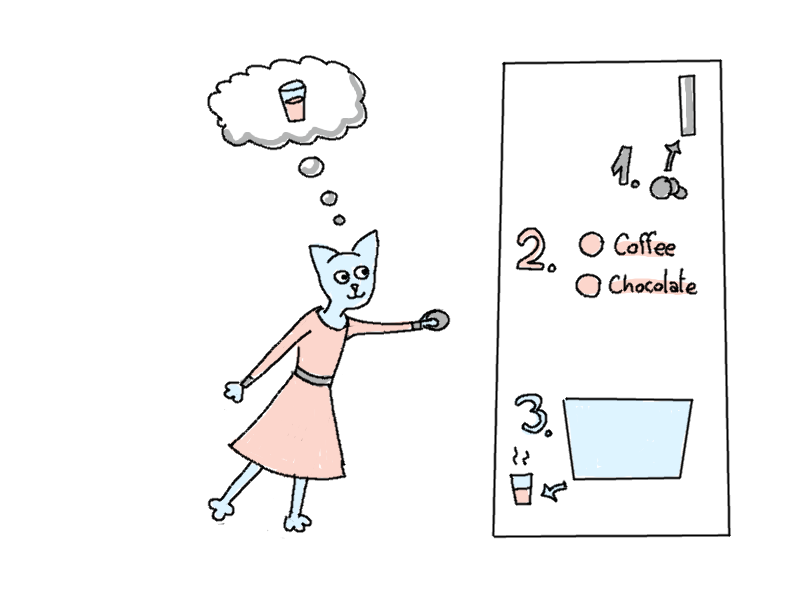
\includegraphics[width=0.6\linewidth]{Pictures/image.png} 
\end{figure}


\section{Einführung}
Im Alltag interagieren wir mit vielen Maschinen, die einfache Programme ausführen. Zum Beispiel, wie viele von euch haben heute den Lift genommen? Oder mussten an einer Ampel anstehen? Oder haben ein Getränk aus dem Automaten vor der Mensa gekauft? Wie werden diese Maschinen gesteuert?

Die Programme, die sie ausführen, haben keine Variablen und keine Datenablage. Man nennt solche Programme \textbf{endliche Automaten}. Heute werden wir Beispiele von endlichen Automaten kennenlernen und diesen Begriff  mathematisch formulieren. Auf dieser Basis werden wir dann in den nächsten Wochen aufbauen und beweisen, welche Probleme lassen sich mit solchen Programmen lösen und welche nicht.

\begin{example}
Eine Ampel kann als endlicher Automat betrachtet werden. Am Anfang ist sie rot, nach einer gewissen Zeit wird sie (zumindest in Deutschland) rot-gelb, dann wird sie grün, dann gelb und schliesslich wird sie wieder rot und der Zyklus geht von vorne los. Schematisch können wir das Verhalten dieser Ampel mit einem gerichteten Graphen darstellen. Wir zeichnen einen Knoten für jede Ampelfarbe und verwenden gerichtete Kanten, um zu zeigen, wie sich die Farben ändern.
\begin{figure}[H]
\centering
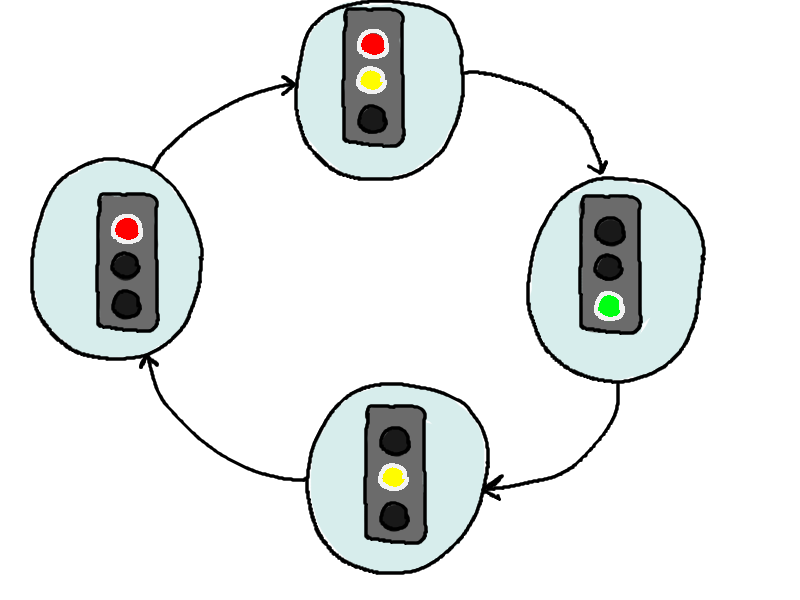
\includegraphics[width=0.4\linewidth]{Pictures/Ampel.png} 
\end{figure}
\end{example}

\begin{example}
Betrachten wir einen Getränkeautomat, welcher Münzen im Wert von 1 CHF erwartet und ein Glas Kaffee oder heisse Schokolade ausschenkt, je nachdem welche Taste gedruckt wurde.
\begin{figure}[H]
\centering
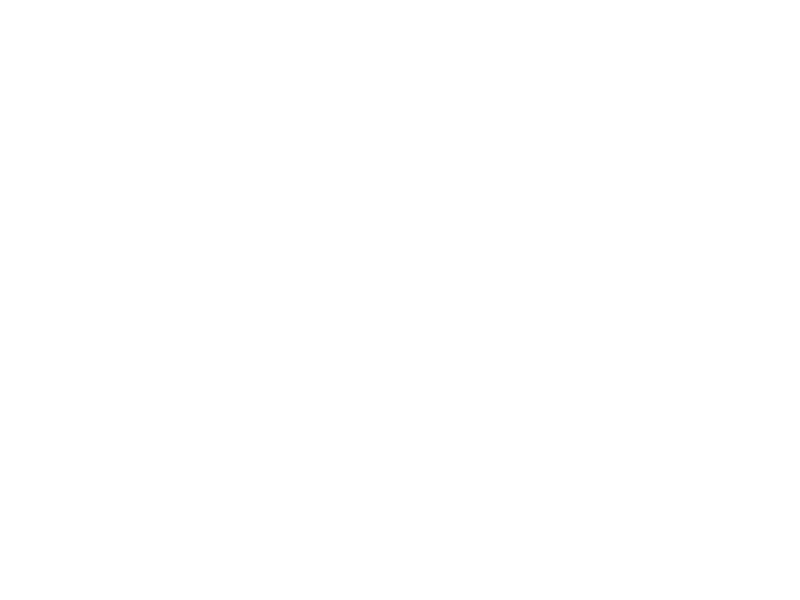
\includegraphics[width=0.6\linewidth]{Pictures/weiss.png} 
\end{figure}
\end{example}

\begin{examplesolution}
\begin{figure}[H]
\centering
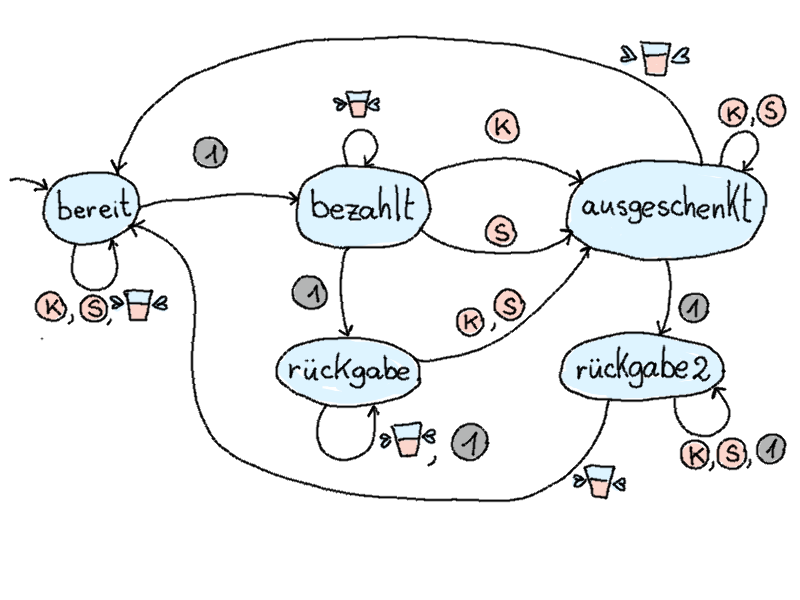
\includegraphics[width=0.6\linewidth]{Pictures/Getraenkeautomat.png} 
\end{figure}
\end{examplesolution}

\begin{question}
Zeichne schematisch einen Obstautomaten, welcher Münzen im Wert von 1 CHF oder 0.5 CHF erwartet und einen Apfel oder eine Orange zurückgibt, je nachdem, welche Taste gedruckt wurde. Jede Frucht kostet 1 CHF. Wie beim Getränkautomaten im obigen Beispiel, behandle auch die Fälle, wenn die Tasten zu früh gedruckt werden, oder wenn Münzen unerwartet eingeworfen werden, oder wenn das Ausgabefensterchen zu früh kontrolliert wird.
\begin{figure}[H]
\centering
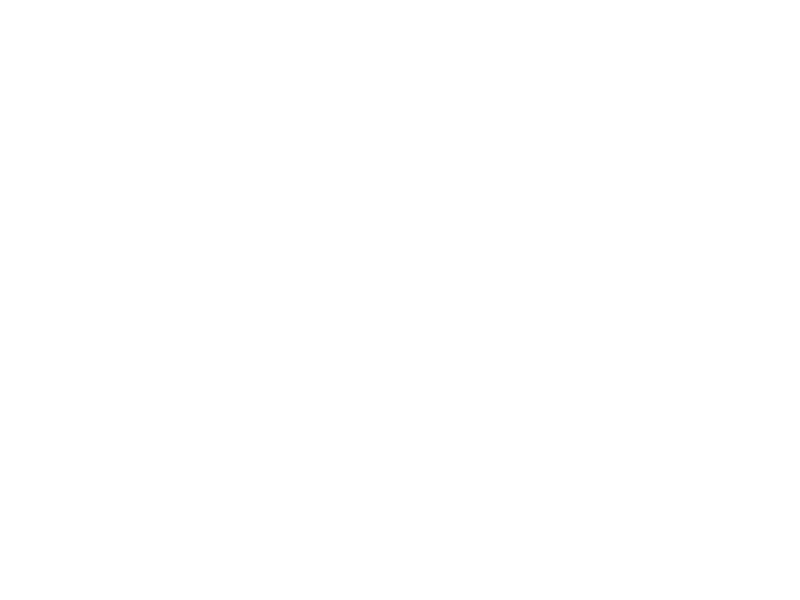
\includegraphics[width=0.6\linewidth]{Pictures/weiss.png} 
\end{figure}
\end{question}

Wir haben bereits 3 endliche Automate gesehen. Was haben sie alle gemeinsam? Welche Informationen brauchen wir, um einen bestimmten Automaten genau nachbauen zu können?\\


\blank[width=\linewidth]{Zustände, Übergänge, mögliche Eingaben, Anfang}
In den folgenden Abschnitten werden wir versuchen, diese Informationen mathematisch zu formulieren. Eine mathematische Formulierung ist nützlich, weil sie ermöglicht, solche Automaten eindeutig zu beschreiben und Aussagen darüber zu beweisen.

\section{Alphabete, Wörter, Sprachen}
Eine wichtige Komponente von einem endlichen Automaten ist die erwartete Eingabe. In diesem Abschnitt befassen wir uns mit dessen mathematischen Formulierung.

\begin{definition}
Eine endliche nichtleere Menge \(\Sigma\) heisst \textbf{Alphabet}. Die Elemente eines Alphabets werden \textbf{Buchstaben}, \textbf{Zeichen} oder \textbf{Symbole} genannt.
\end{definition}

\begin{example}
\begin{enumerate}[(a)]
    \item \(\Sigma_{tast} = \{a, b, \dots, z, A, B, \dots, Z, 0, \dots, 9, ., ,, !, ?, -, :, \dots, @\}\) ist das Alphabet aller Zeichen, die sich mit einer Tastatur eintippen lassen. Wir benutzen dieses Alphabet, um Texte oder Programme zu schreiben.
    \item \(\Sigma_{bin} = \{0, 1\}\) ist das Alphabet, in welchem binäre Zahlen dargestellt werden.
    \item \(\Sigma_{Morse} = \{.,-\}\) ist das Alphabet der Morsezeichen.
\end{enumerate}
\end{example}

\begin{exercise}
Welche der folgenden Mengen sind Alphabete? Begründe deine Antwort.
\begin{itemize}[label=$\square$]
    \item \(\Sigma = \{a, b, C, D, e, f\}\)
    \item \(\Sigma = \{\}\)
    \item \(\Sigma = \{+, -, \times, \div\}\)
    \item \(\Sigma = \{2, 4, 6, 8, 10, 12, 14, \dots\}\), die Menge aller geraden natürlichen Zahlen
\end{itemize}
\end{exercise}

\begin{exercise}
Welches Alphabet hatten wir für die Eingabe vom Getränkeautomaten benutzt? Und welches hast du für den Obstautomaten verwendet?\\

\blank[width=\linewidth]{}
\end{exercise}

\begin{definition}
Sei \(\Sigma\) ein Alphabet. Ein \textbf{Wort über \(\Sigma\)} ist eine endliche (eventuell leere) Folge von Buchstaben aus \(\Sigma\). Das \textbf{leere Wort \(\lambda\)} ist die leere Buchstabenfolge.
\end{definition}

\begin{example}
\begin{enumerate}[(a)]
    \item Sei \(\Sigma = \{a, b, c\}\). Mögliche Wörter über diesem Alphabet sind \texttt{aaaab}, \texttt{ababc}, \(\lambda\) und \texttt{a}.
    \item Sei \(\Sigma_{Morse} = \{.,-\}\). Mögliche Wörter über diesem Alphabet sind \verb|--|, \verb|---|, \verb|.-.|, \verb|...| und \verb|.|.
\end{enumerate}
\end{example}

\begin{exercise}
Welche der folgenden Buchstabenfolgen sind Wörter über dem Alphabet \(\Sigma = \{a, b, c\}\)? Begründe deine Antwort.
\begin{itemize}[label=$\square$]
    \item \texttt{abbbbcdccca}
    \item \(\lambda\)
    \item \texttt{abab}
\end{itemize}
\end{exercise}

\begin{exercise}[solution=true]
Schreibe zu jeder Symbolfolge jeweils das kleinste Alphabet \(\Sigma\), so dass die Symbolfolge ein Wort über \(\Sigma\) ist.
\begin{enumerate}[(a)]
{\setstretch{1.5}
    \item \texttt{abbabb},\hfill \(\Sigma = \)\blank[width=0.5\textwidth]{\(\{a,b\}\)}
    \item \texttt{01000.(00)!},\hfill \(\Sigma = \)\blank[width=0.5\textwidth]{\(\{0,1,.,(,),!\}\)}
    \item \texttt{aXYabwRS},\hfill \(\Sigma = \)\blank[width=0.5\textwidth]{\(\{a,b,w,R,S,X,Y\}\)}
    
}
\end{enumerate}
\end{exercise}

\begin{definition}
Auf Wörter definieren wir folgende Operationen:
\begin{description}
    \item[Länge:] Sei \(w\) ein Wort über \(\Sigma\). \(\abs{w}\) bezeichnet die Länge des Wortes. Zum Beispiel, \(\abs{\text{aabbcc}}=6\).
    \item[Anzahl Symbole:] Sei \(w\) ein Wort über \(\Sigma\). \(\abs{w}_a\) bezeichnet die Anzahl der Vorkommnisse des Symbols \(a\) im Wort \(w\) des Wortes. Zum Beispiel, \(\abs{\text{aaabbc}}_a=3\).
    \item[Konkatenation:] Seien \(v\) und \(w\) zwei Wörter über \(\Sigma\). \(vw\) bezeichnet das Wort, welches mit \(v\) anfängt und mit \(w\) endet. Man bezeichnet \(v\) als Präfix und \(w\) als Suffix von \(vw\). Zum Beispiel, wenn wir \texttt{001} mit \texttt{01} konkatenieren, erhalten wir \texttt{00101}.
    \item[Wiederholung:] Sei \(a \in \Sigma\) und \(n \in \mathcal{N}\). \(a^n\) bezeichnet das Wort, welches aus \(n\) Wiederholungen von \(a\) besteht. Zum Beispiel, \(\text{0}^4\) bezeichnet das Wort \texttt{0000}.
\end{description}
\end{definition}

\begin{definition}
Eine (eventuell leere) Menge von Wörtern über einem Alphabet \(\Sigma\) bezeichnen wir als eine \textbf{Sprache über \(\Sigma\)}. 
\end{definition}

\begin{exercise}
Bei den folgen Beispielen von Sprachen, entscheide, ob die Sprache endlich viele oder unendlich viele Wörter enthält. Ausserdem schreibe auf jeweils ein Wort über dem angegebenen Alphabet, welches in der Sprache und eins, welches \emph{nicht} in der Sprache ist.

{\setstretch{2}
\begin{enumerate}[(a)]
    \item \(L = \{x \in \{0,1\}^* \mid \abs{x}_0 \leq 3 \text{ und } \abs{x}_1 \in \{1,2\}\}\) \\
    \blank[width=\linewidth]{}

    \item \(L = \{wabba \in \{a,b\}^* \mid w \in \{a, b\}^* \text{ und } \abs(w)_a \leq 3\}\) \\
    \blank[width=\linewidth]{}
    
    \item \(L = \{0^n 1^n \in \{0, 1\}^* \mid n \in \mathcal{N}\}\) \\
    \blank[width=\linewidth]{}
\end{enumerate}
}
\end{exercise}

\begin{exercise}
Schreibe die folgenden informell beschriebenen Sprachen formal als Mengen auf.


\begin{enumerate}[(a)]
    \item Die Sprache aller Wörter über \(\Sigma_{tast}\), die mit drei Ausrufezeichen enden.\\
    {\setstretch{1.5} 
    
    \blank[width=\linewidth]{}}

    \item Die Sprache aller Wörter über \(\{A, C, G, T\}\), welche höchstens 4 \(C\)'s enthalten und in denen die Summe der Anzahlen von \(A\)'s und \(G\)'s genau \(10\) ist. \\
    {\setstretch{1.5} 
    
    \blank[width=\linewidth]{}}
    
    \item Die Sprache aller Wörter über \{a, b, c\}, welche mit dem Präfix \(a^3 b^2 c\) anfangen. \\
    {\setstretch{1.5} 
    
    \blank[width=\linewidth]{}}
\end{enumerate}
\end{exercise}

\section{Matematische Formulierung eines endlichen Automates}
\begin{definition}[solution=true]
Ein \textbf{endlicher Automat} ist ein Quintupel \(M = (Q, \Sigma, \delta, q_0, F)\), wobei:
{\setstretch{1.5} 
\begin{enumerate}[(i)]
    \item \(Q\) \blank[width=0.5\linewidth]{eine endliche Menge von \textbf{Zuständen} ist,}
    \item \(\Sigma\) \blank[width=0.5\linewidth]{das \textbf{Eingabealphabet} ist,}
    \item \(q_0 \in Q\) \blank[width=0.5\linewidth]{der \textbf{Anfangszustand} ist,}
    \item \(F \subseteq Q\) \blank[width=0.5\linewidth]{die \textbf{Menge der akzeptierenden Zustände} ist,}
    \item \(\delta:\) \blank[width=0.5\linewidth]{\(Q\times \Sigma \rightarrow Q\) die \textbf{Übergangsfunktion} ist.}
\end{enumerate}
}
\end{definition}

\begin{example}
In diesem Beispiel beschreiben wir mathematisch den Getränkeautomat.
{\setstretch{1.5} 
\begin{enumerate}[(i)]
    \item \(Q =\) \blank[width=0.5\linewidth]{}
    \item \(\Sigma =\) \blank[width=0.5\linewidth]{}
    \item \(q_0 =\) \blank[width=0.5\linewidth]{}
    \item \(F =\) \blank[width=0.5\linewidth]{}
    \item \(\delta:Q \times \Sigma \rightarrow Q \) die Übergansfunktion.
    Wir können alle Werte von \(\delta(q,a)\) für alle \(q \in Q\) und für alle \(a \in \Sigma\) in eine Tabelle schreiben.
        \begin{figure}[H]
\centering
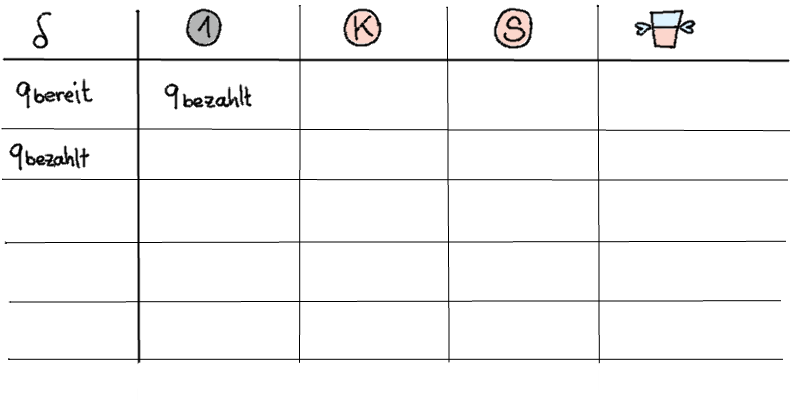
\includegraphics[width=\linewidth]{Pictures/Getraenkeautomat_table.png} 
\end{figure}
\end{enumerate}
}
\end{example}

\begin{exercise}
Formuliere mathematisch den Obstautomaten. Für die Übergangsfunktion kannst du eine Tabelle benutzen analog zum vorherigen Beispiel.
\begin{figure}[H]
\centering
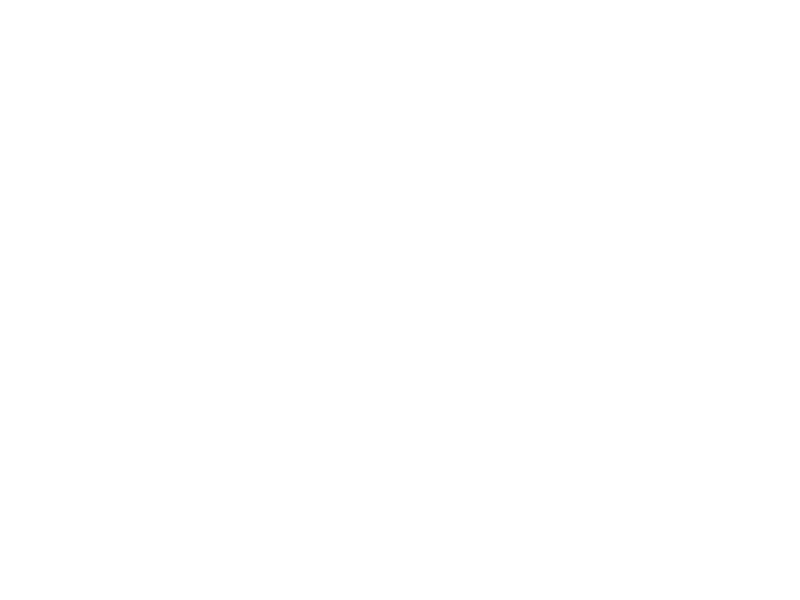
\includegraphics[width=\linewidth]{Pictures/weiss.png} 
\end{figure}
\end{exercise}


\section{Zusammenfassung}
In diesem Kapitel haben wir \textbf{endliche Automaten} kennengelernt. Endliche Automaten werden zum Beispiel eingesetzt, um Ampel an Kreuzungen, Lift oder Snackautomaten zu steuern.

Endliche Automaten haben eine endliche Anzahl \textbf{Zustände}. Sie bearbeiten sequentiell eine \textbf{Eingabe} und können nach jedem Symbol in einen anderen Zustand übergehen. Die \textbf{Zustandsübergänge} hängen nur vom aktuellen Zustand und vom eingelesenen Symbol ab.

Bevor jegliche Eingabesymbole eingelesen werden, befindet sich ein endlicher Automat in seinem \textbf{Anfangszustand}. Nach der vollständigen Bearbeitung einer Eingabe endet der endliche Automat entweder in einen \textbf{akzeptierenden Zustand} (in diesem Fall wurde die Eingabe akzeptiert) oder in einen nicht-akzeptierenden Zustand (in diesem Fall wurde die Eingabe verworfen).

Die Eingabe zu einem endlichen Automat ist ein \textbf{Wort} über seinem \textbf{Eingabealphabet}. Ein \textbf{Alphabet} ist eine endliche nicht-leere Menge von \textbf{Symbolen}. Ein \textbf{Wort über einem Alphabet} ist eine (möglicherweise leere) Folge von Symbolen aus dem Alphabet. Eine \textbf{Sprache über einem Alphabet} ist eine (möglicherweise leere) Menge von Wörter über diesem Alphabet.

\end{document}